\documentclass[11pt, oneside]{article} 
\usepackage[margin=3.4cm]{geometry} 
\geometry{letterpaper}
\usepackage{graphicx}
\usepackage{hyperref}
\usepackage{amssymb}
\usepackage{caption}
\usepackage{float}
\usepackage{setspace}
\usepackage{esvect}
\usepackage{url}
\usepackage[section]{placeins}

%\setcounter{secnumdepth}{0}
\onehalfspacing

\newcounter{refno}
\newcommand{\reflabel}[1]{\refstepcounter{refno}\label{#1}[\arabic{refno}]}  %create ref labels in-text

\newcommand{\refinit}[1]{\noindent \hangindent=0.6cm [\ref*{#1}]}  %citation initialization in reference section

\begin{document}
% Title Page
\begin{titlepage}
	\newcommand{\HRule}{\rule{\linewidth}{0.5mm}}
	
	\center
	\textsc{\LARGE University of Calgary}\\[1.5cm]
	\textsc{\Large ENGO 651: Advanced Geospatial Topics}\\[0.5cm]
	\textsc{\large Final Project}\\[0.5cm]

	\HRule\\[0.4cm]
	{\huge\bfseries Fuellytics: Real-Time Vehicular Fuel Consumption and Emissions Monitoring}\\[0.4cm]
	\HRule\\[1.5cm]
	
	{\large\textit{Group 2}}\\
	Adam \textsc{Smith} (30031453)\\
	Chavisa \textsc{Sornsakul} (30193209)\\
	Wai Ka \textsc{Wong Situ} (30184219)\\
	
	\vfill\vfill\vfill
	{\large \today}
	
	\vfill\vfill\vfill
	
\includegraphics[width=8cm,]{img/schulich.png}\\[1cm]	
\end{titlepage}

\section{Executive summary}
Next to oil and gas, the transportation sector is the second largest emitter of greenhouse gases in Canada.  Since 1990, Canadian greenhouse gas emissions from transportation have increased by over 32\%, and this is largely driven by increases from passenger vehicles \reflabel{canadaghg}.  Mitigating these emissions is crucial to reducing the harmful effects of climate change on the environment and protecting our natural landscapes.

Monitoring fuel consumption is vital to understand the efficiency of a vehicle and its impact on the environment.  This data can provide valuable insights into the effects of driving style, conditions, and vehicle type on a vehicle's emissions, and incentivize the driver to adapt their driving style to reduce total greenhouse gas emissions and fuel costs.  

Our innovative new smartphone application, \textit{Fuellytics}, utilizes the smartphone's inertial and GPS sensors to measure fuel consumption and emissions of various greenhouse gases in real-time.  Fuellytics helps drivers track their fuel costs by monitoring velocity and acceleration while driving, and displaying the current and total fuel use for the current trip on an interactive frontend.  Moreover, the user is able to track their routes, and analyze the emissions of various greenhouse gases including carbon dioxide, nitrous oxides, particulate matter, and unburned hydrocarbons on current and previous routes.

The dynamic frontend of Fuellytics is built using the JavaScript library React-Native \reflabel{reactnative} to enable simplified development and cross-platform compatibility.  To alllow for easy user authentication and provide versatile development tools, the backend is written with the Python library Django \reflabel{django}.

Explain a little more about architecture here...

Mention results and briefly mentions lessons learned here...



\section{Problem statement}
According to the International Energy Agency, transportation accounts for almost one-quarter of global greenhouse gas emissions, and within that, road transport is responsible for the largest share of emissions \reflabel{transport-emissions}.  The burning of fossil fuels in vehicles produces, along with several other pollutants, carbon dioxide, which is the most prevalent greenhouse gas contributing to global warming.  Although electric vehicles are becoming more popular in the developed world, still 91\% of all transport relies on oil-based products such as gasoline, which is only a 3\% drop from the early 1970's \reflabel{oil-based-transport}.  Reducing carbon emissions from vehicles is crucial to mitigate the harmful effects of climate change and reduce the environmental burden of vehicular transport.

Tracking vehicle fuel consumption is essential to understanding the amount of carbon emissions produced by vehicles. Fuel consumption data can provide valuable insights into the efficiency of a vehicle and its impact on the environment, and can also provide insights to the driver about their driving style and fuel costs.  However, fuel consumption is heavily dependent on various factors such as vehicle type, terrain, and driving style, making it difficult to measure over short time periods.  According to the US Department of Energy, obeying speed limits, accelerating and braking gently, and reading the road ahead can improve fuel economy by up to 30\% on highways and up to 40\% in stop-and-go traffic \reflabel{driving-style}.  Moreover, engine size, vehicle weight, and driving in hilly or mountainous areas can drastically increase fuel consumption and, consequently, carbon emissions.  Some modern vehicles are equipped with a dashboard gauge that displays fuel consumption while driving, however, these gauges are often vague and uninformative, usually showing nothing more than an unlabelled bar or dial which increases while accelerating.  Without a means to directly monitor fuel consumption, drivers are often left unaware of their fuel use and how their driving style and driving conditions can be altered to reduce their vehicle's impact on the environment.

The presented smartphone application, \textit{Fuellytics}, provides an innovative solution to monitoring fuel consumption and greenhouse gas emissions in real-time, and provides insights and reports to drivers about their fuel use while driving as well on previous trips.  Fuellytics helps drivers better understand the environmental impacts of their vehicle, make educated decisions regarding transportation, and save money on fuel.

\section{Similar solutions and available literature}

For industrial applications, several fleet management solutions exist that offer analytics on fuel consumption and tracking.  For example, \textit{FuelForce Fuel Management Systems} \reflabel{fuel-force} provides tools to monitor, track, view, and analyze fuel use of fleet vehicles, and \textit{Triscan} \reflabel{triscan} provides a similar functionality by integrating their systems with refuelling stations. These solutions, however, are targeted at industrial applications, and do not provide real-time analytics to the driver.  Moreover, these and similar tools are focused around fleet management and cost savings, and often do not provide an analysis of environmental impact.

Multiple applications for personal use exist which track fuel usage over long periods of time to determine fuel costs and fuel economy. The web and iOS application \textit{Fuelly} \reflabel{fuelly} allows users to enter volume and cost data each time they refuel to gain insight into their fuel consumption and fuel costs over time.  A similar application, \textit{FuelLine} \reflabel{fuelline}, was recently developed by a team at BCIT and additionally contains a routing feature to predict fuel costs on future routes.  Notably, these solutions differ from Fuellytics in that they do not provide real-time fuel consumption data while driving and they are focused more on monitoring costs rather than reducing environmental impacts.

Some applications developed for carbon emission tracking, such as \textit{MyEarth} \reflabel{myearth} and \textit{Carbon Footprint \& CO2 Tracker} \reflabel{capture}, provide functionality to track CO$_2$ emission in many categories including travel.  However, the main focus of these applications is tracking carbon emissions in a broad range of categories, not an in-depth and real-time analysis of carbon emissions and fuel use from driving.

A 2019 paper \reflabel{main-paper} from the North China University of Technology utilized the vehicle specific power (VSP) distribution to predict fuel consumption in real-time from velocity and acceleration data using a binned linear regression approach.  Their model achieves a relatively low error while requiring only velocity, acceleration, engine displacement, and the presence or absence of a supercharger or turbocharger as input.  However, the road surface is assumed flat, so road gradient is not included in the model.

\reflabel{tank2wheel} and \reflabel{analytic-fc} both derive more sophisticated models for the real-time fuel consumption and emissions of light-duty vehicles.  These models provide more accurate results than the model described in [\ref*{main-paper}], but require knowledge of many parameters specific to the vehicle such as rotational internal inertia of the engine, the selected gear, the tire radius, and the total loaded weight.  These parameters are generally unknowable in our application.  Other methods, such as those described in \reflabel{wvu-ai} and \reflabel{fc-phone}, compute fuel consumption post-trip using various methods, but lack a real-time fuel consumption analysis, so are unsuitable for our application.

As such, Fuellytics uses an adaptation of the method described in [\ref*{main-paper}] as the basis for the numerical prediction of real-time fuel consumption.  This model was chosen due to its simplicity, relatively low error, and availability of the model parameters.  Modification of the model to account for road gradient is also easily implemented.

\section{Solution summary}

Our innovative application, \textit{Fuellytics}, is a cutting-edge smartphone application that enables drivers of light-duty passenger vehicles to track their fuel consumption and CO$_2$ equivalent emissions in real-time.  After creating an account and registering their vehicle, users can log their trips, and the app collects data on location, acceleration, and angular velocity from the sensors embedded in the smartphone while driving.  Fuellytics utilizes this data to compute the rates of fuel consumption and pollutant production and displays this information in an interactive user interface to provide insights regarding the user's fuel use and environmental impact. 

The application not only displays emissions and fuel consumption information, but also tracks their current location and displays their trip on an interactive map.  Furthermore, the user can view and analyze fuel consumption and CO$_2$ emissions from previously logged trips, and see their previous routes on a map. These statistics allow users make educated decisions about their driving and transportation habits and adjust their driving style to improve fuel economy and save money.  Moreover, they highlight the environmental impact of their vehicle use to promote environmentally friendly transportation choices.

\section{Architecture}

\subsection{Design rationale}

\subsection{Architecture description}

\subsection{API}

\subsection{Sequence Diagram}

\subsection{Data models and JSON encodings}

\section{Results}
Upon opening Fuellytics, the user is presented with a login page (Figure \ref*{fig:login-register}) showing the Fuellytics logo and fields for the user to enter their credentials, as well as a login button. If the user attempts to login with invalid or missing credentials, the login attempt will fail.  A successful login will bring the user to the home page of the application.

If the user is not yet registered, they can select the register button to be brought to the registration page shown in Figure \ref*{fig:login-register}.  To register, the user must provide a username (containing at most 150 characters) and email (with valid email formatting) which are not already associated with an account, and a password with a minimum length of 8 characters.  If these requirements are not met, the registration will fail. Upon successful registration, the user will automatically be logged in and brought to the application home page, shown in Figure \ref*{fig:homepage}.
\begin{figure}[H]
\centerline{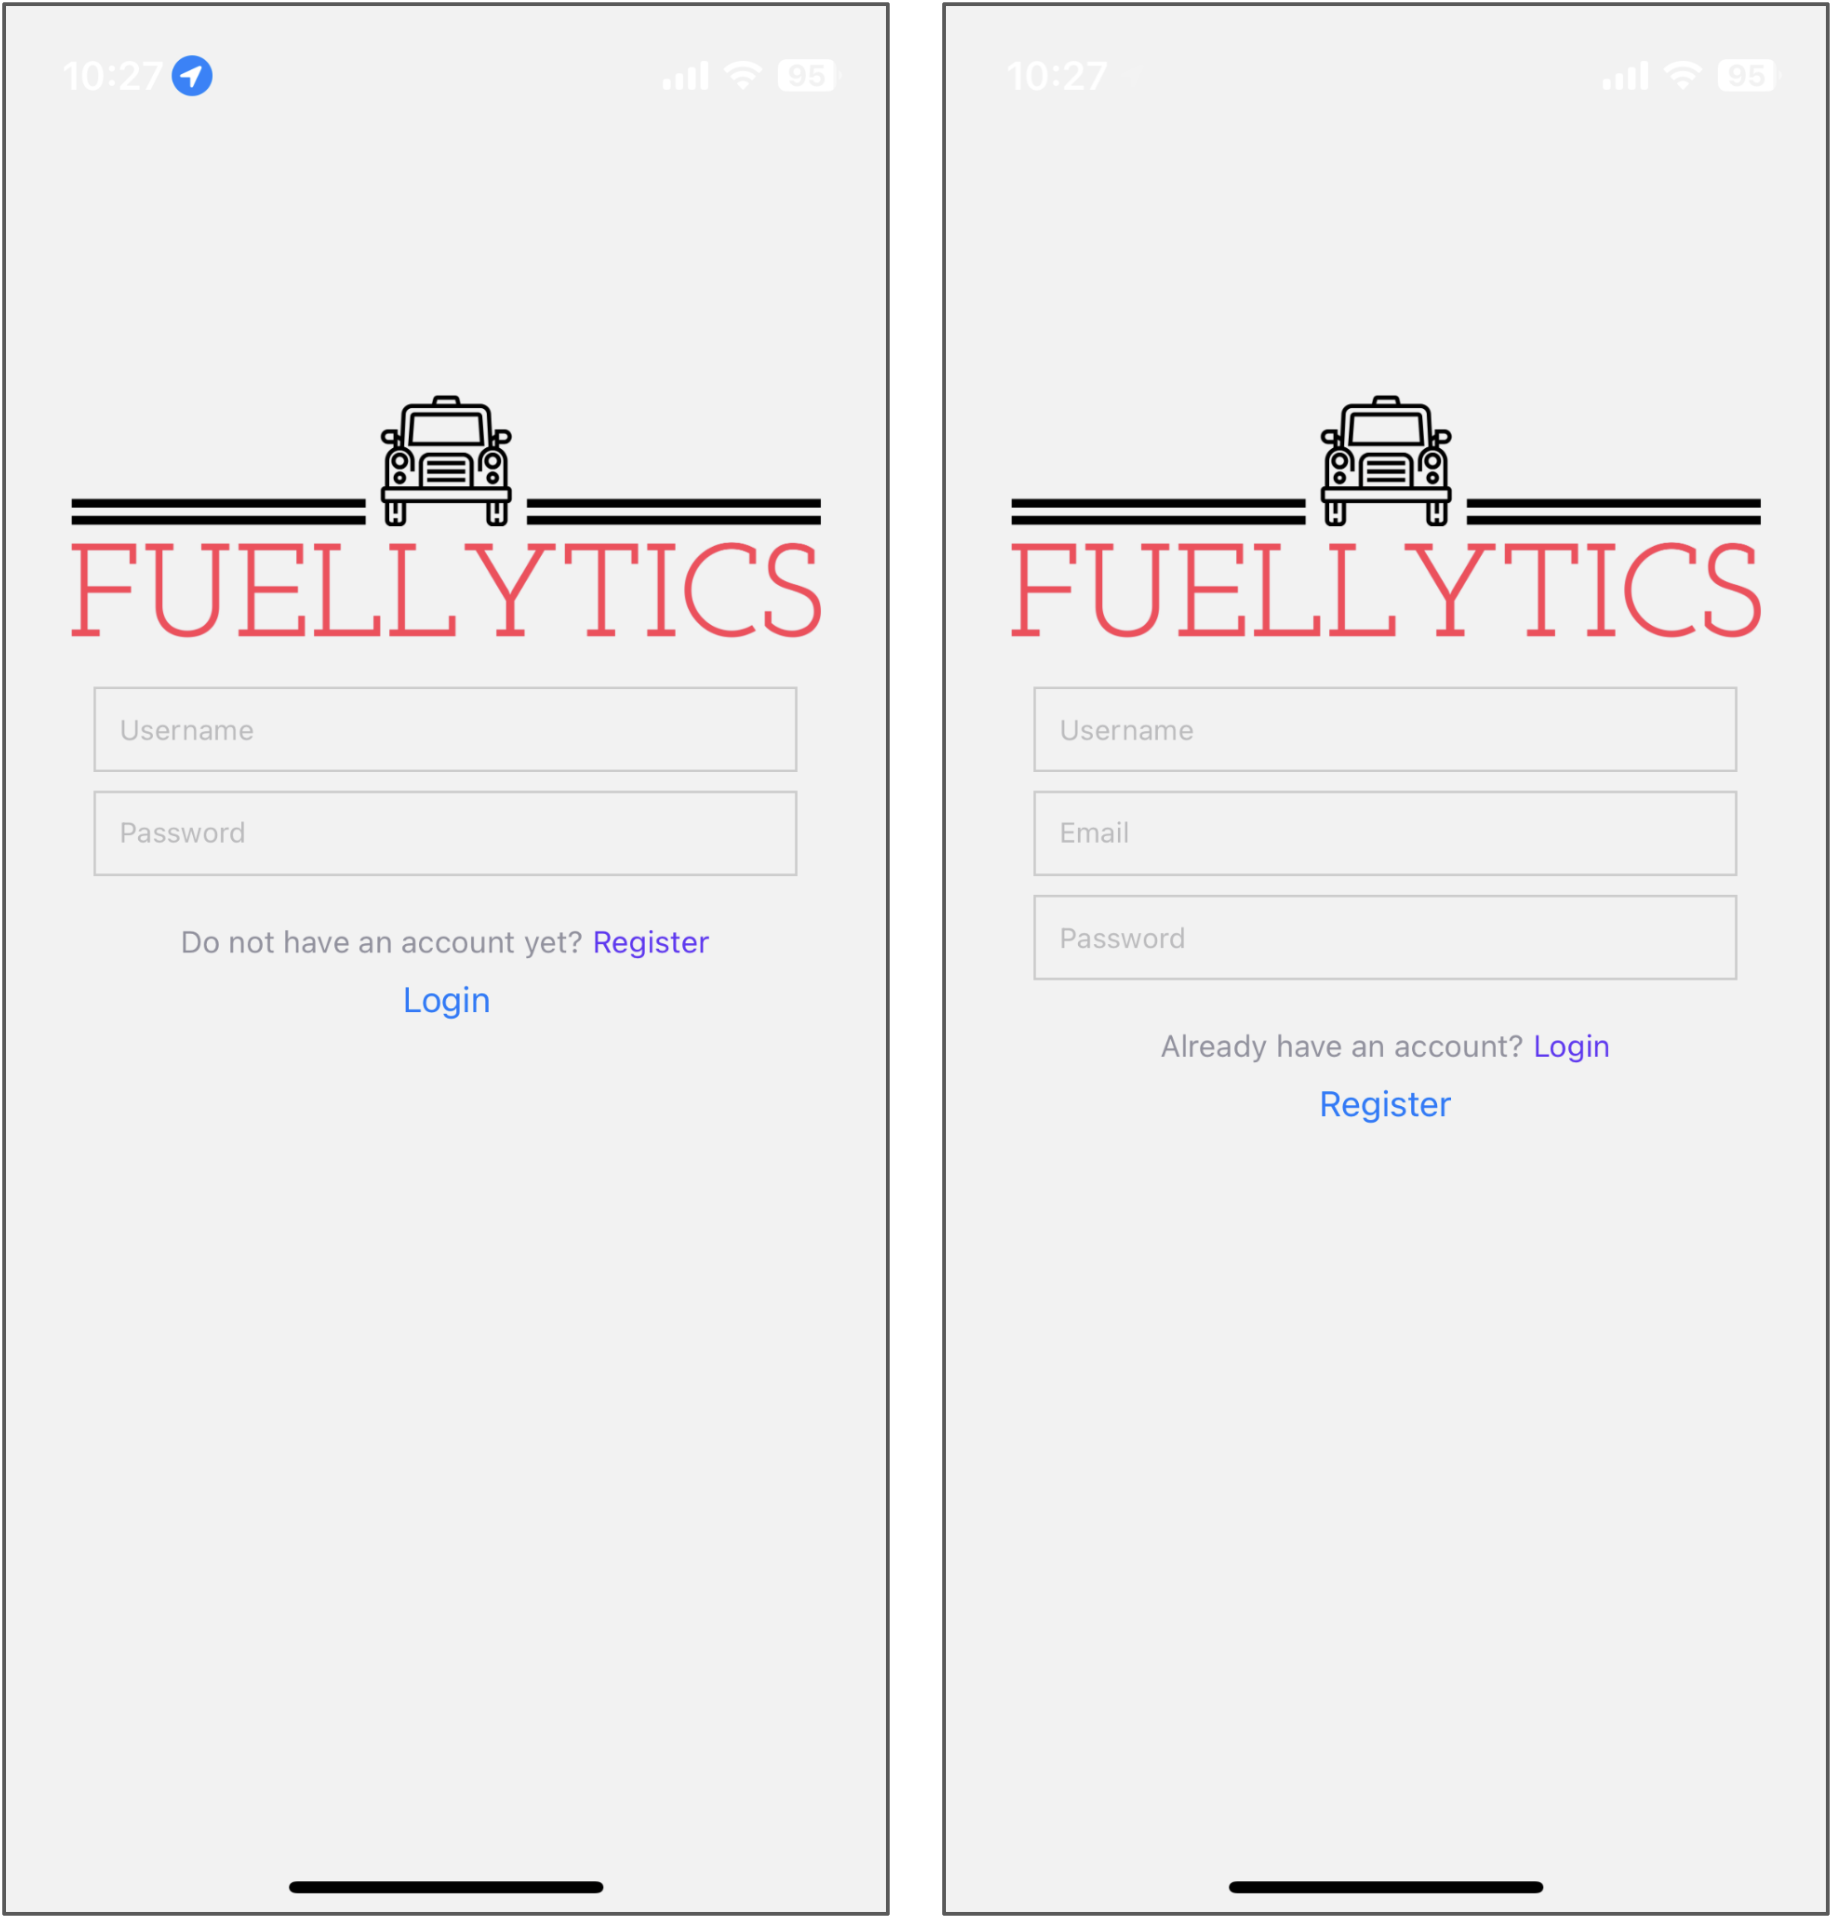
\includegraphics[width=11cm]{img/login-register.png}}
\caption{\label{fig:login-register} Login page (left) and registration page (right) of the Fuellytics application.}
\end{figure}

On the home page the user is greeted with a welcome message, and the list of vehicles that the user has added to their account is displayed.  If there are no vehicles associated with the user's account, the message ``No vehicles registered.'' is displayed.  A logout button is available in the top left corner of the page.

The user can easily remove vehicles by selecting the `x' icon next to the vehicle name. Vehicles can be added by selecting the ``Add new vehicle'' button above the navigation bar.  This brings up a popup where the user can search for their vehicle by typing in the search field and then create the vehicle profile by selecting the ``Create'' button.  ******************Fuellytics has data for over 22,000 unique vehicles, however, if the user's vehicle is not available, the user can manually enter their vehicle's credentials after selecting the ``Enter my own vehicle'' button.  The credentials required by Fuellytics are the engine displacement of the vehicle, whether or not the vehicle is supercharged or turbocharged, and, optionally, the vehicle's mass and the product of the drag coefficient and frontal area. [NOT IMPLEMENTED YET]******************
\begin{figure}[H]
\centerline{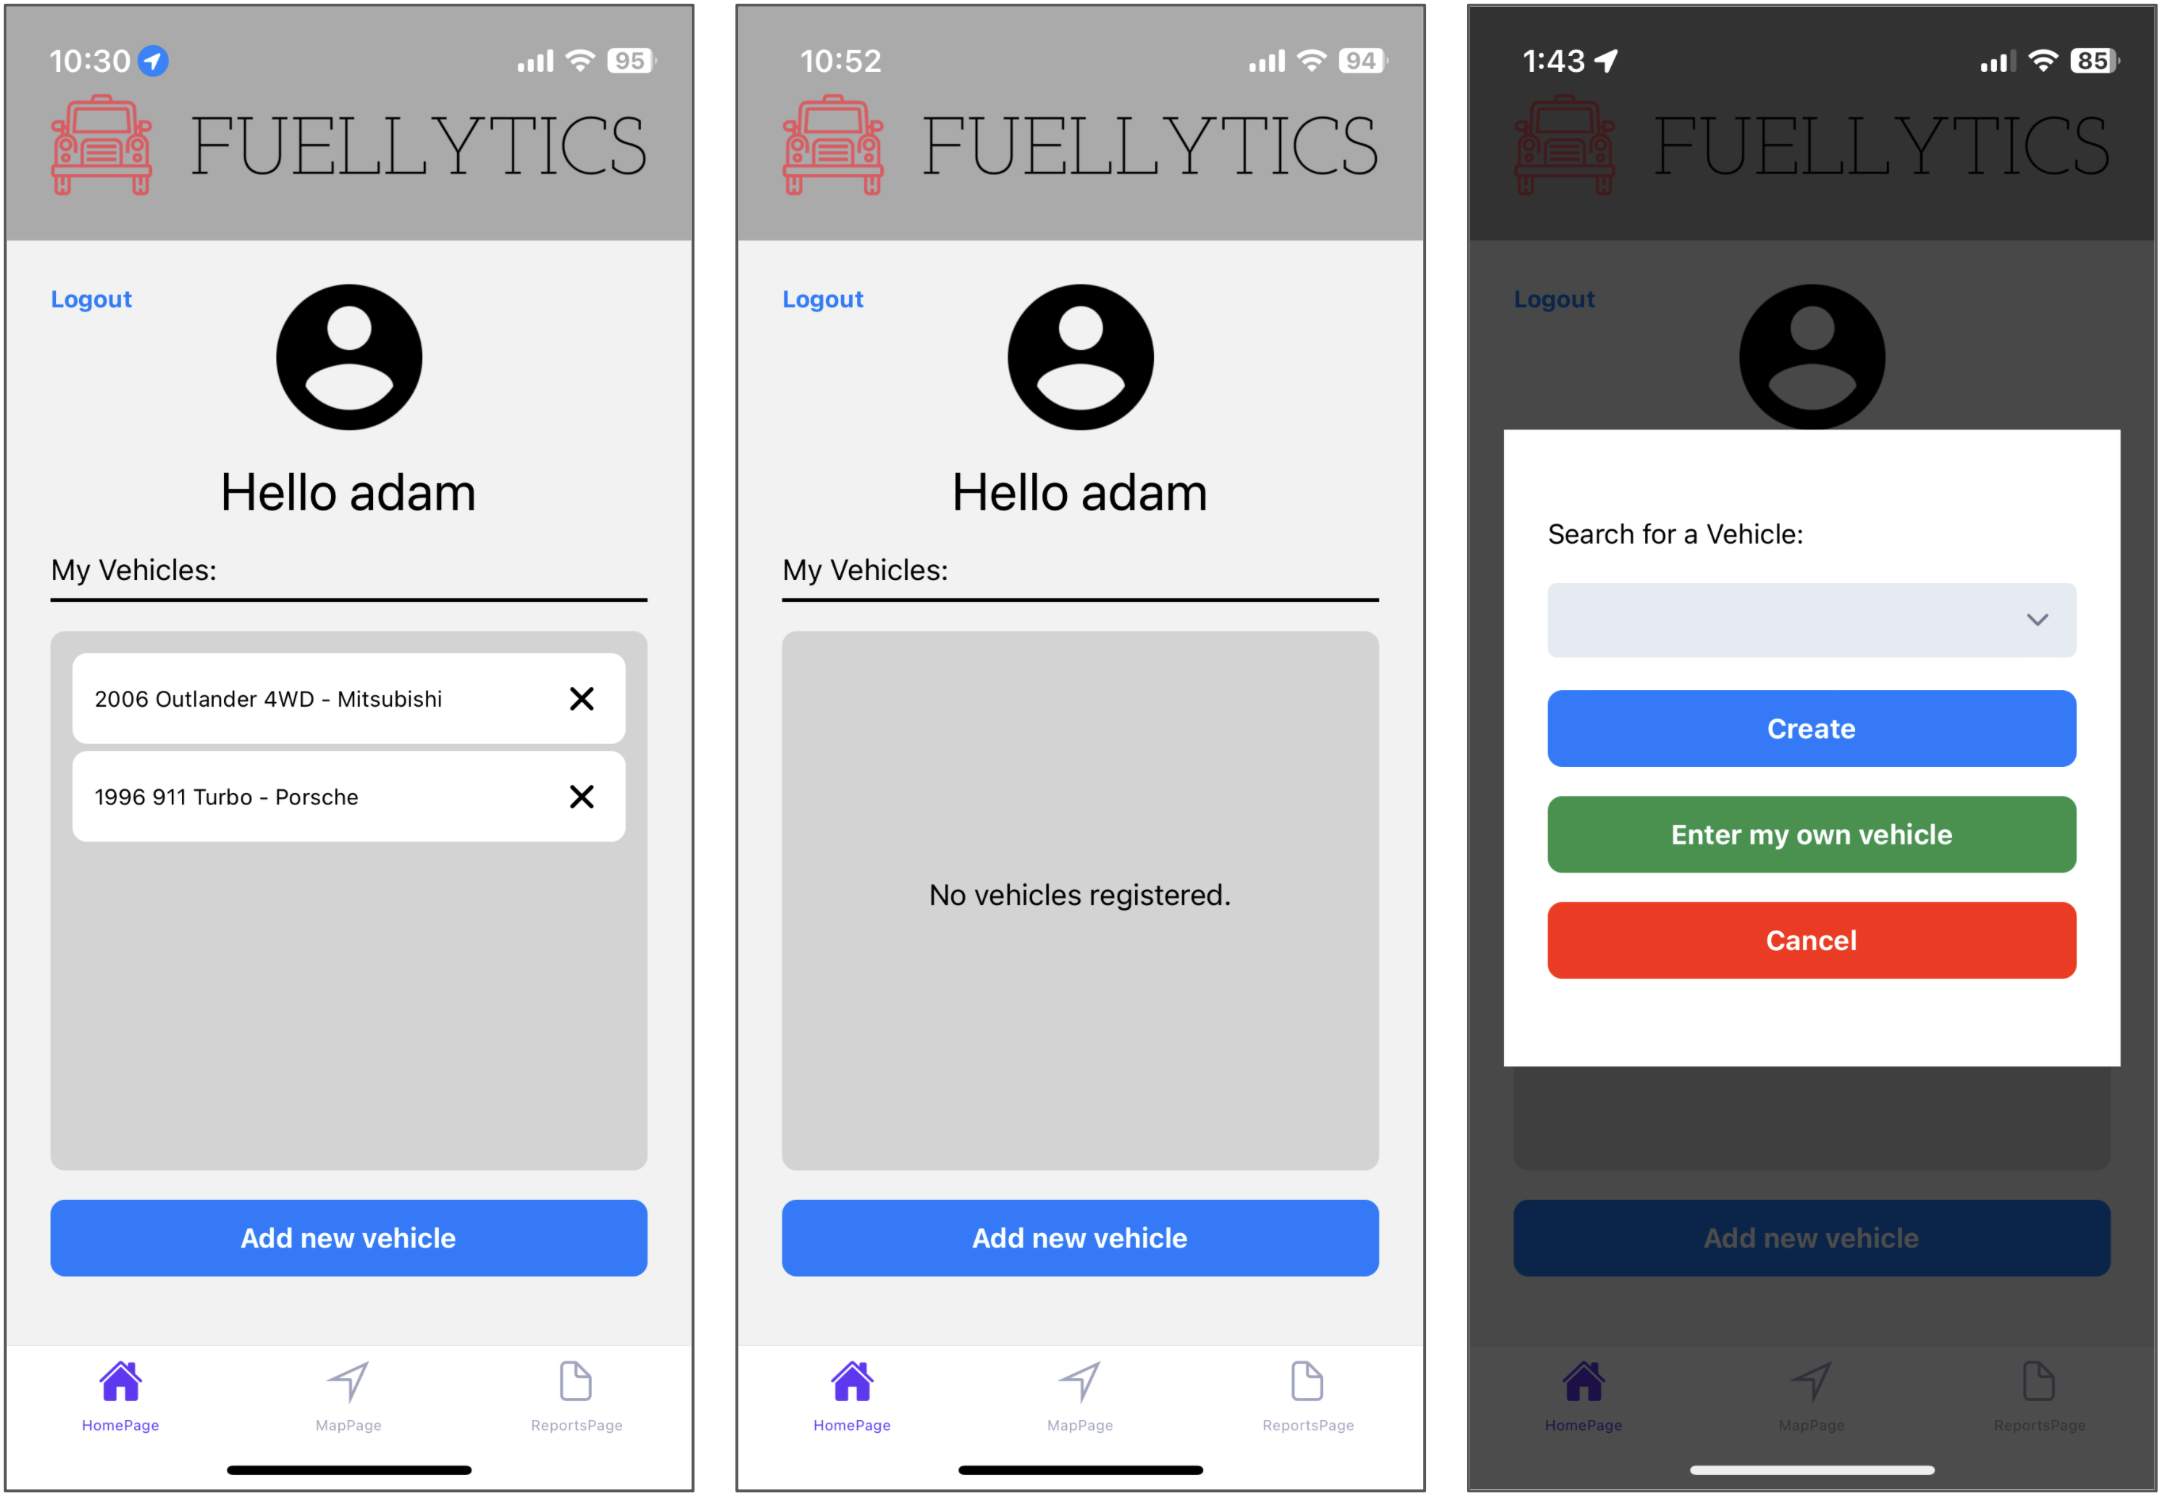
\includegraphics[width=16.5cm]{img/homepage.png}}
\caption{\label{fig:homepage} The Fuellytics home page with (left) and without (middle) vehicles added to the user's account. The right image shows the popup for adding a new vehicle.}
\end{figure}

A navigation bar at the bottom of the page allows for easy navigation throughout the Fuellytics application.

The map page, shown in Figure \ref*{fig:mappage}, is where users can begin recording their routes and tracking their fuel consumption and carbon emissions.  The user can select their vehicle from the vehicles associated with their account from the dropdown menu.  Initially, the ``Start recording'' button will be hidden and a ``Connecting...'' message will be displayed.  Once the GPS connection has been established and location data is being received, the ``Start recording'' button will become visible, and it will become clickable once a vehicle is selected from the dropdown.

Selecting the ``Start recording'' button will begin a trip recording.  Figure \ref*{fig:recording} shows the screens displayed during a trip recording.  These screens contain an interactive map which tracks the user's location in real-time.  A pin is placed on the map showing the users current location, and their track is shown as a black polyline which updates as they move.  A panel slides up from the bottom of the page to reveal plots of the current CO$_2$ emissions of the vehicle in mL/s, the current fuel consumption in mL/s, and the current vehicle speed in km/h.  These plots dynamically update every second, and show data for the last minute.  At any time, the recording can be paused by selecting the ``Pause Recording'' button, and continued by selecting ``Continue Recording''.  
\begin{figure}[!t]
\centerline{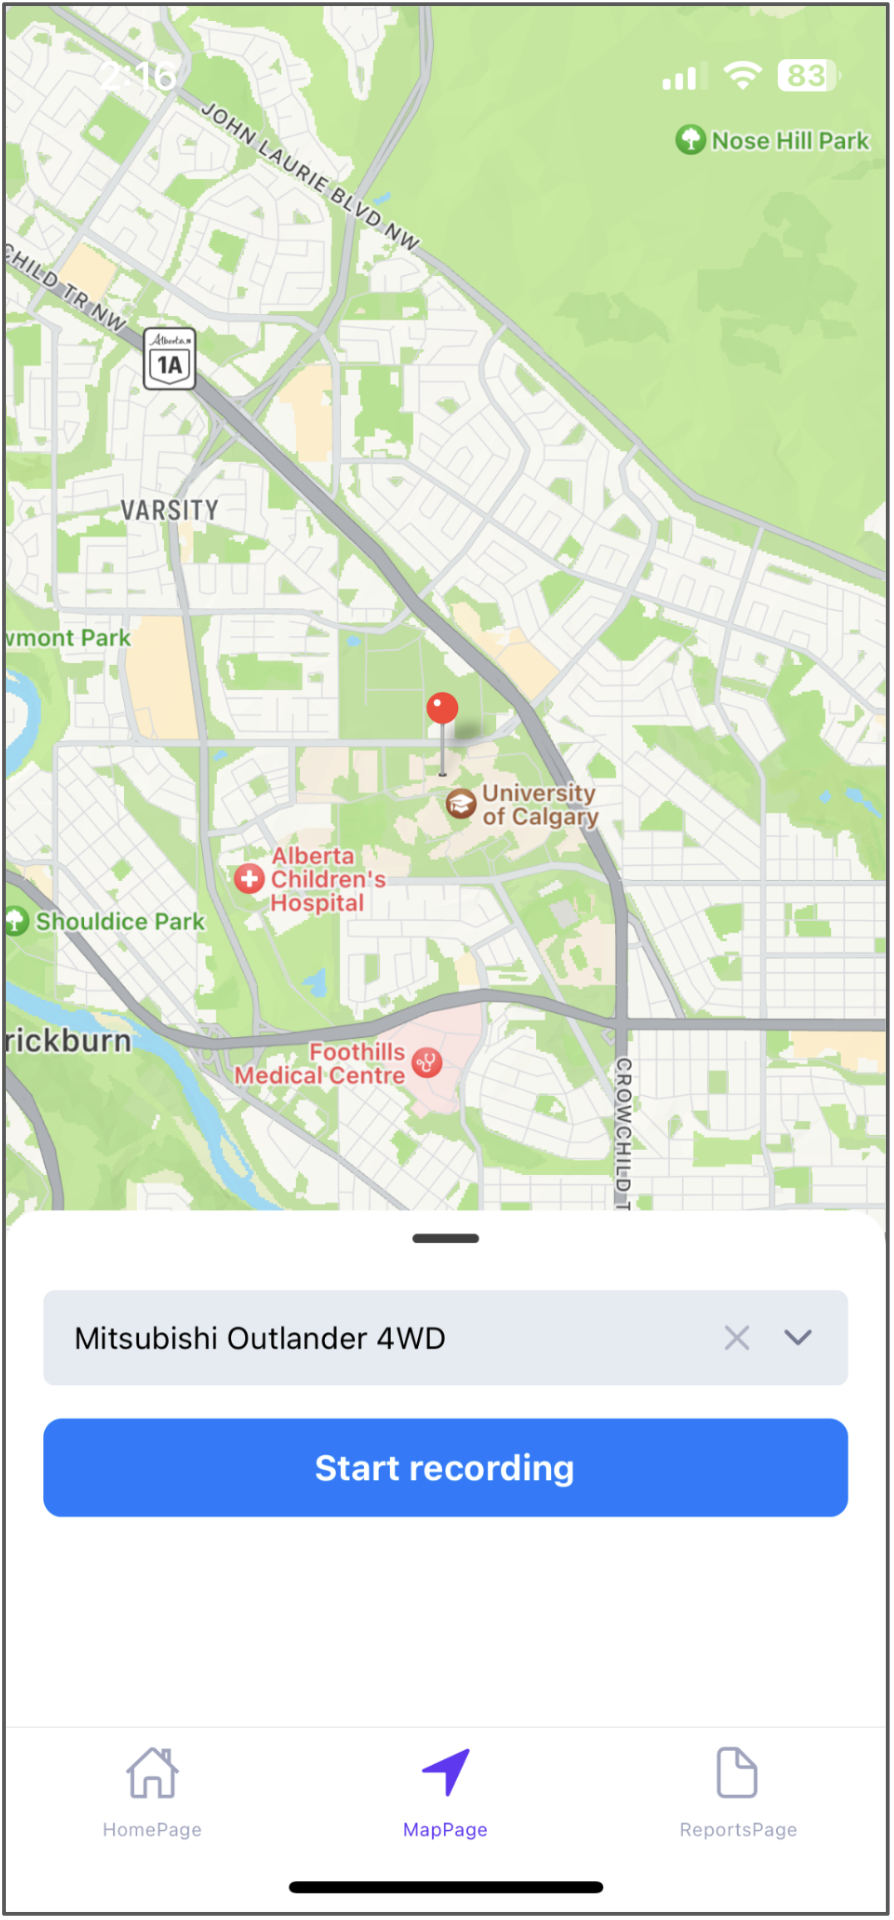
\includegraphics[width=5.5cm]{img/mapinit.png}}
\caption{\label{fig:mappage} The map page where the user can begin a trip recording.}
\end{figure}
\begin{figure}[H]
\centerline{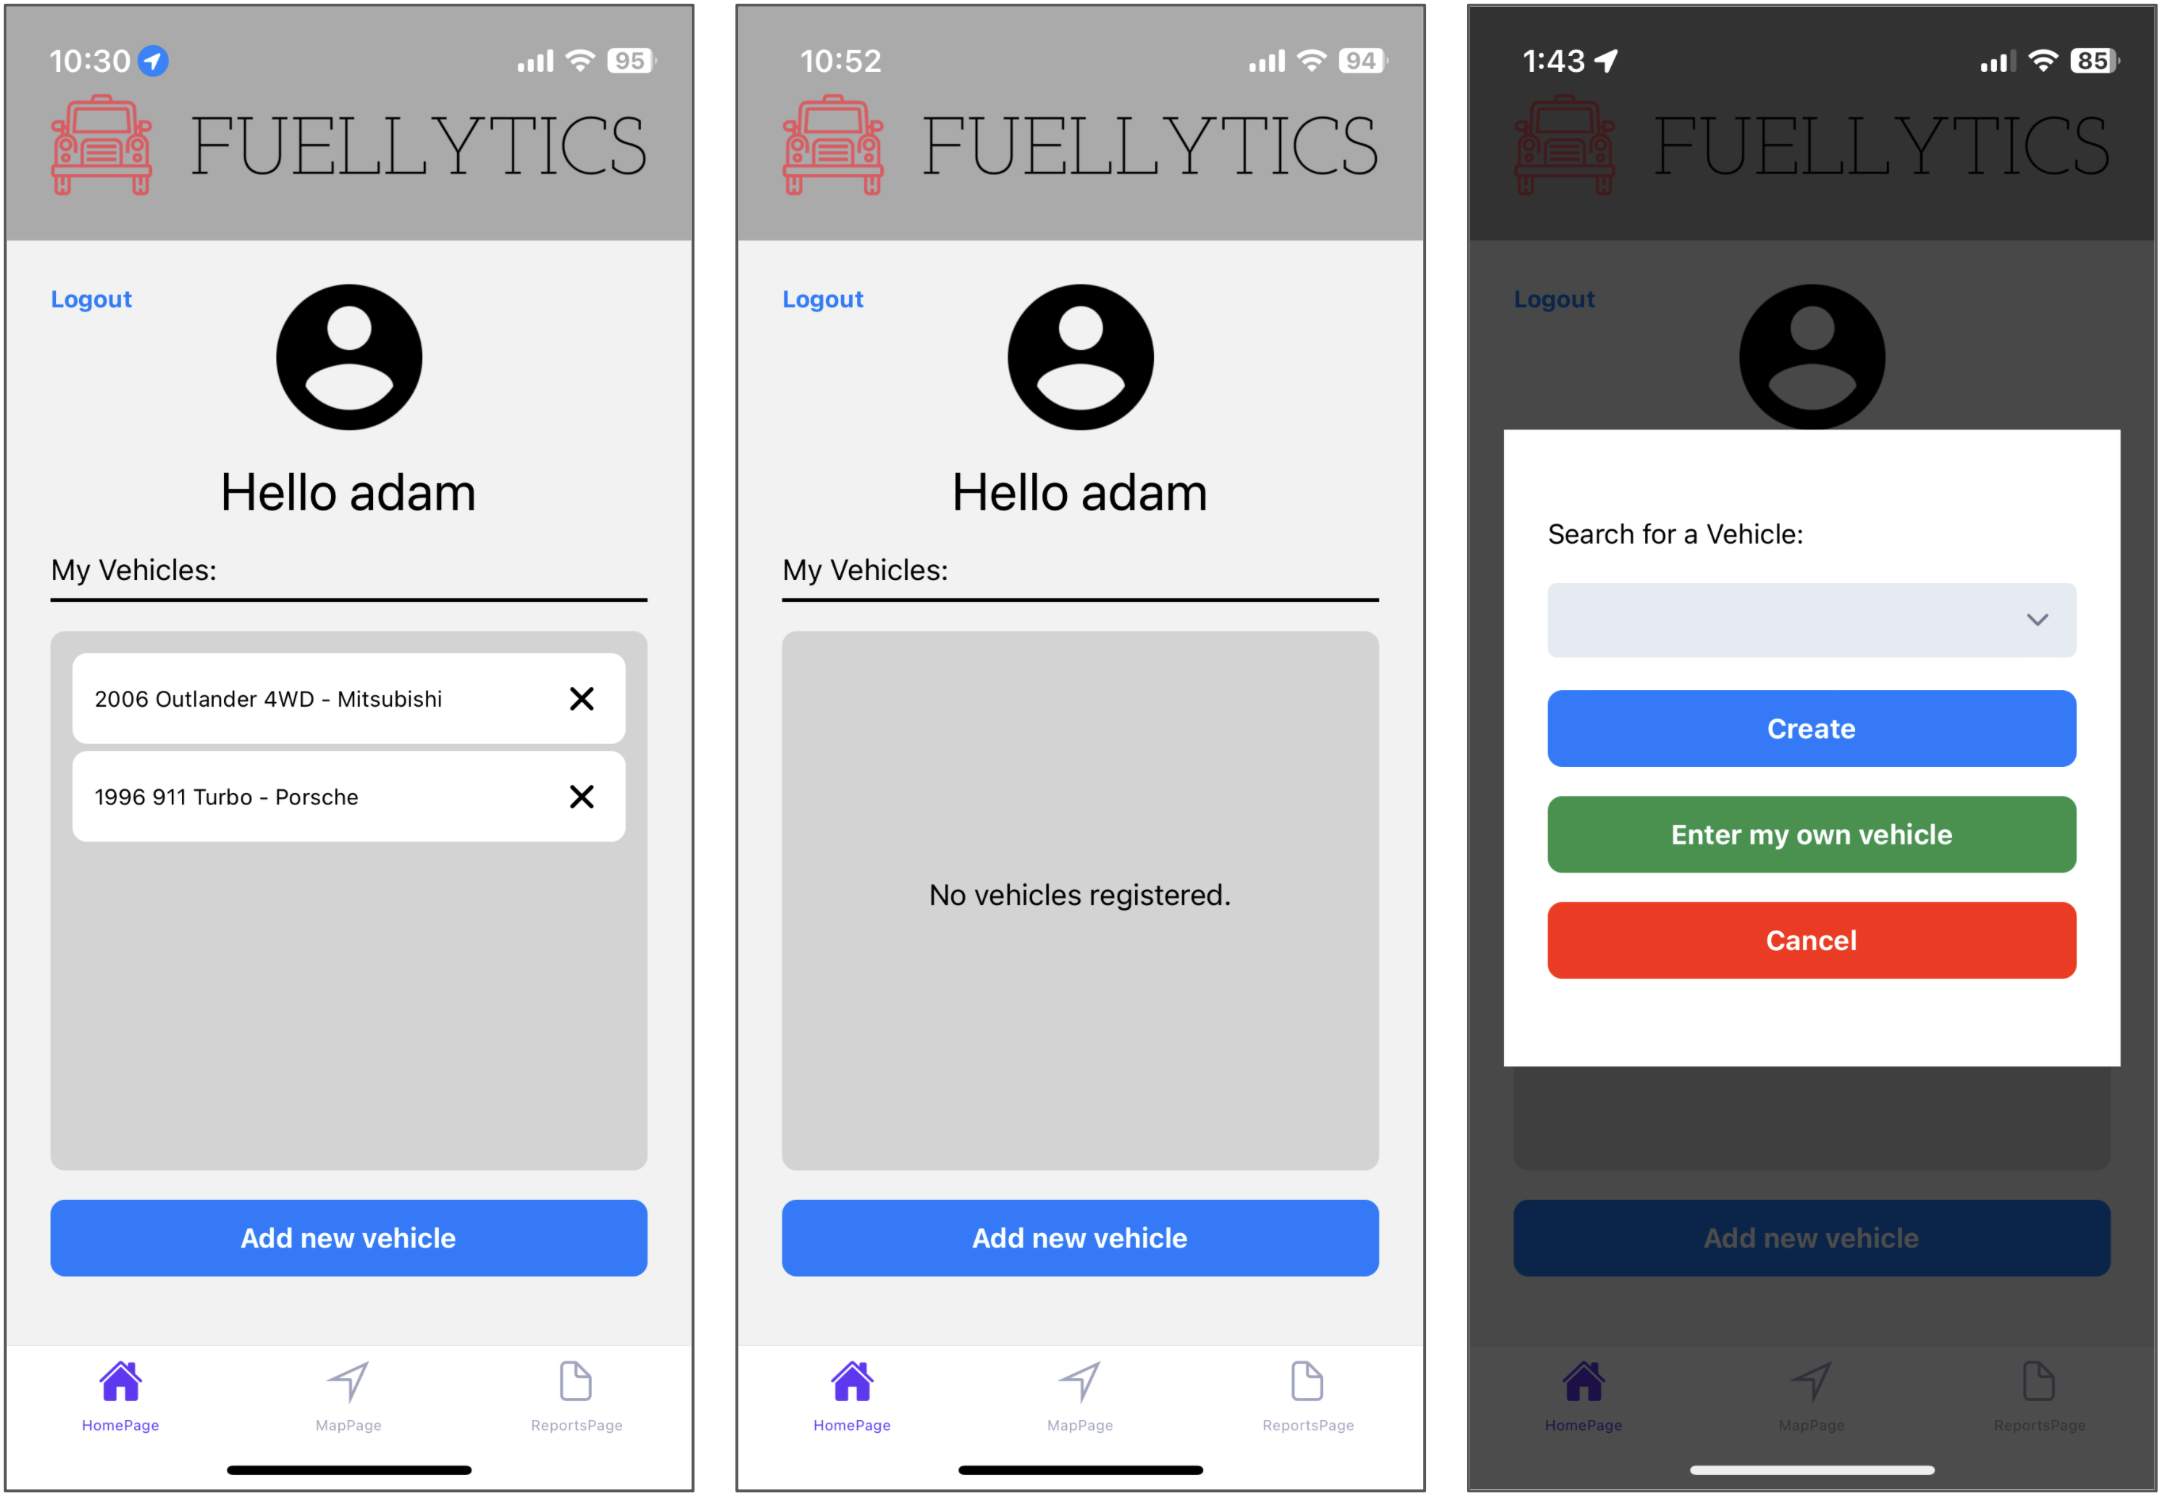
\includegraphics[width=16.5cm]{img/homepage.png}}
\caption{\label{fig:recording} REPLACE FIGURE WITH IMAGES OF RECORDING.}
\end{figure}

Once the user arrives at their location, the ``End Recording \& Save'' button will finalize the trip recording and save it.  As shown in Figure \ref*{fig:confirmation}, a confirmation page will appear with a summary of the trip including the elapsed time, the total gas consumption, and the total CO$_2$ emissions. Selecting the ``Back'' button brings the user back to the map page.
\begin{figure}[H]
\centerline{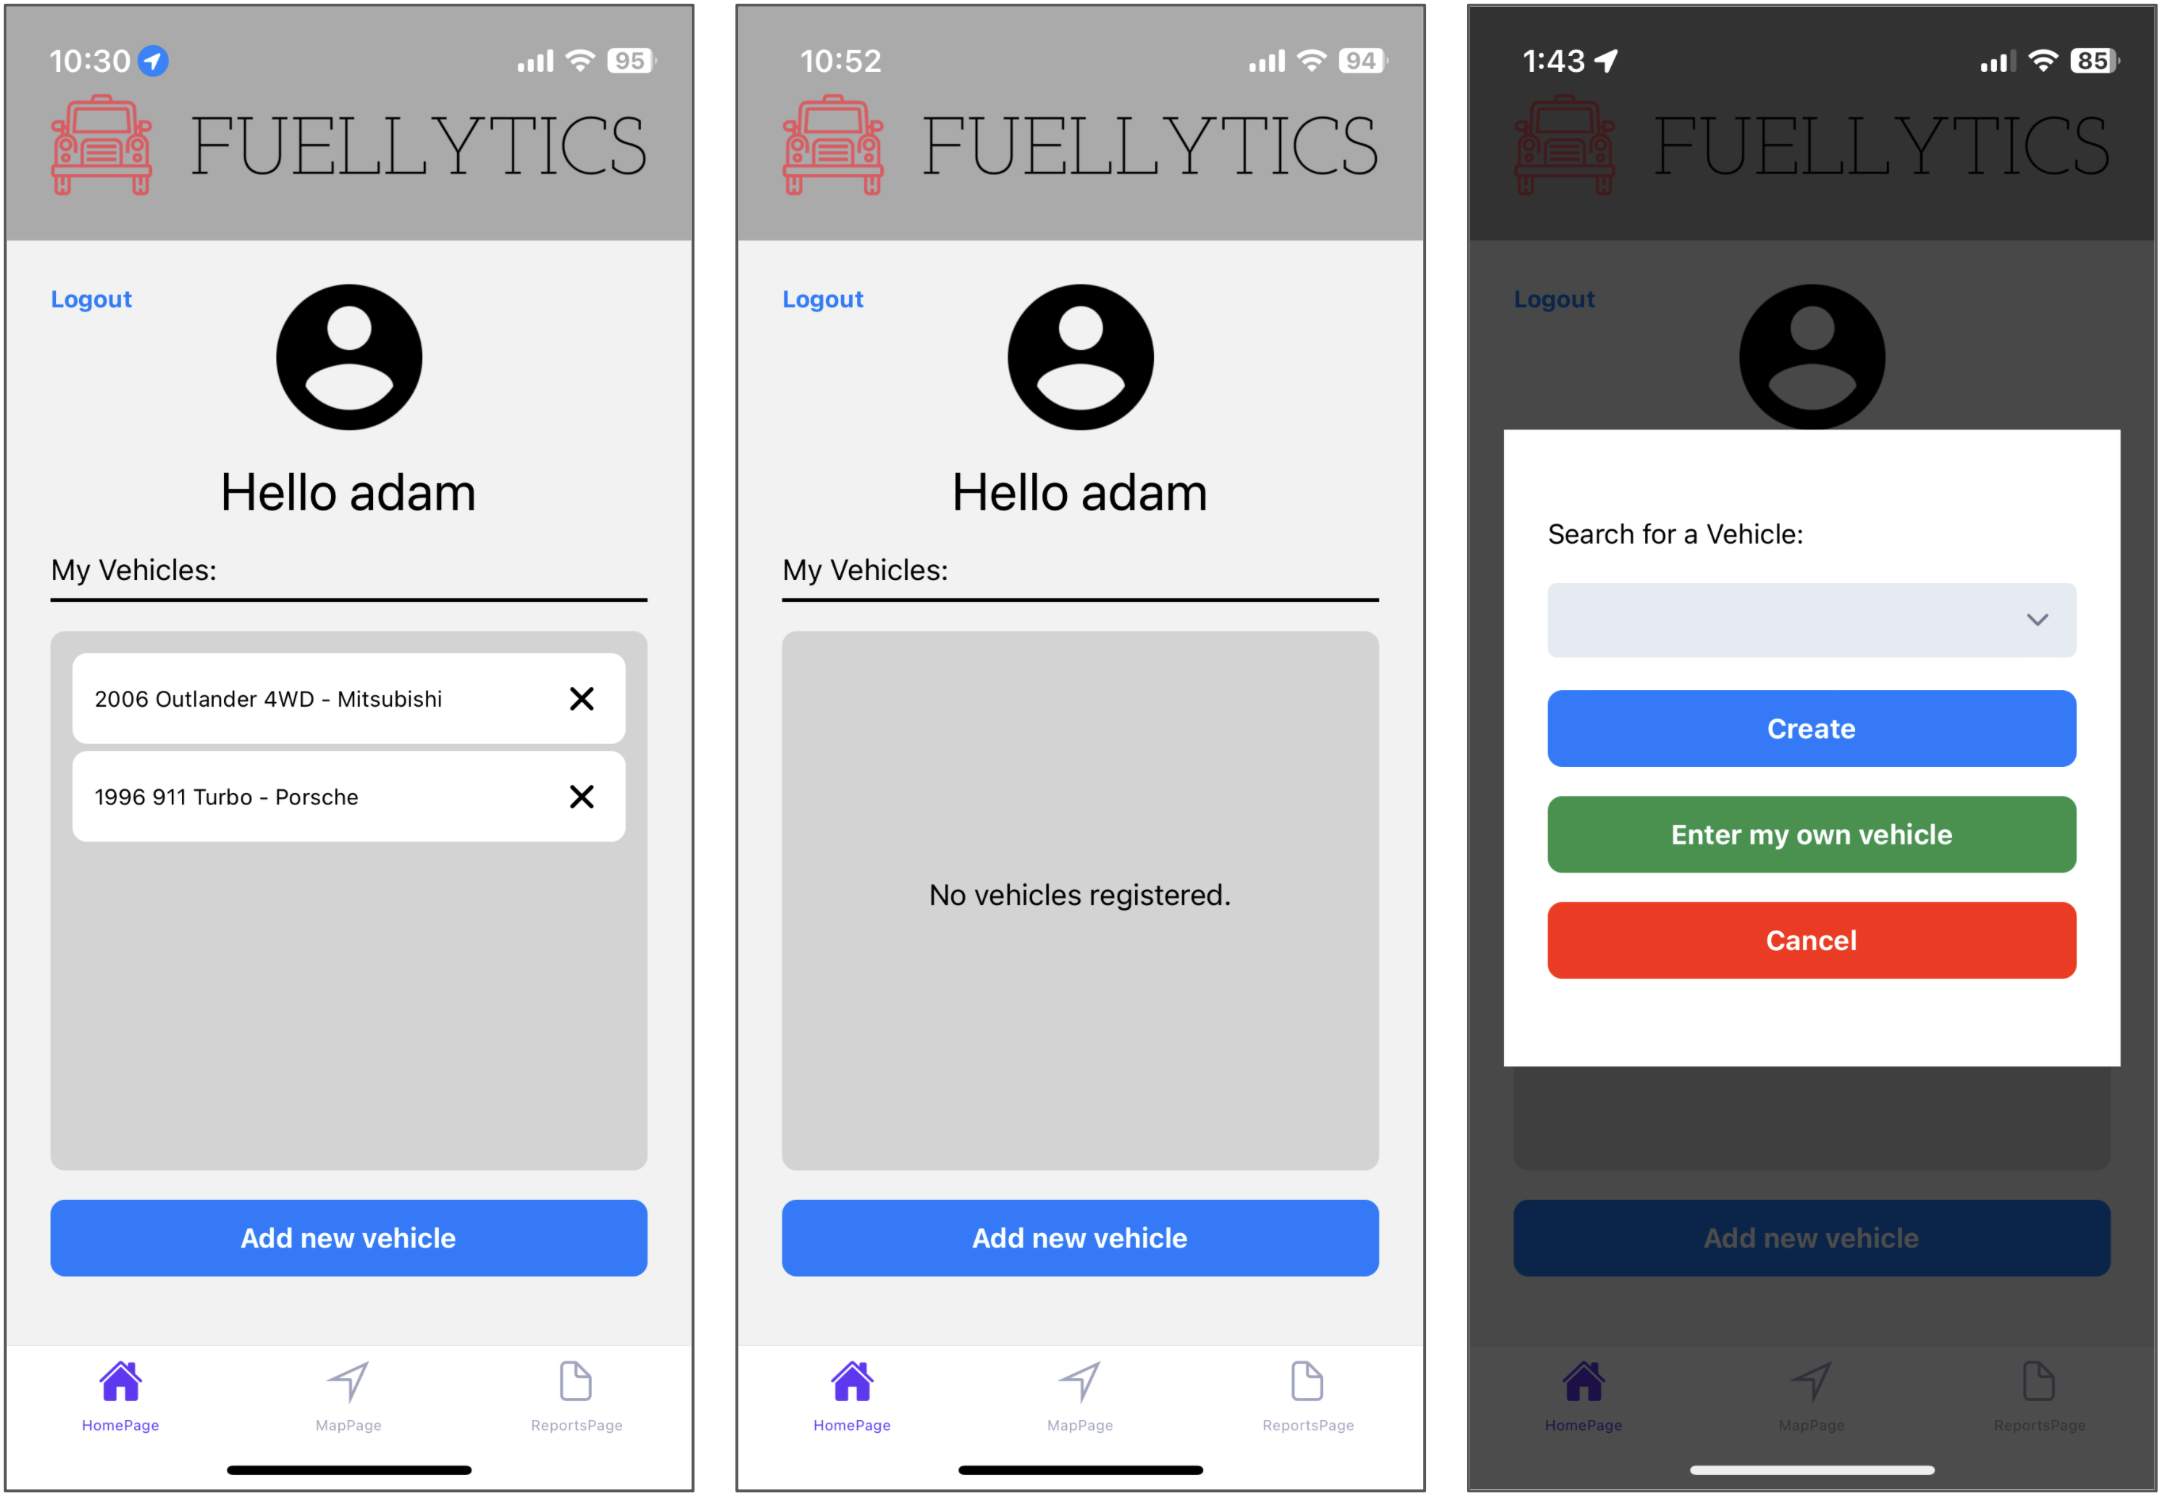
\includegraphics[width=16.5cm]{img/homepage.png}}
\caption{\label{fig:confirmation} REPLACE FIGURE WITH IMAGE OF CONFIRMATION PAGE.}
\end{figure}

Summaries of the users trips are available on the reports page, shown in Figure \ref*{fig:reports}.  Here, all of the users past trips appear in a scrollable list. The calendar icon above the trip list opens a date range selector widget to filter the trip list within a specified date range. Selecting a trip reveals the trip information page to show further information about the trip including the start and end times, the vehicle used, the total CO$_2$ emissions, the total fuel consumption, and the average speed.  An interactive map is also displayed showing the vehicle route. The user can return to the trips page by selecting the ``Back'' button.
\begin{figure}[H]
\centerline{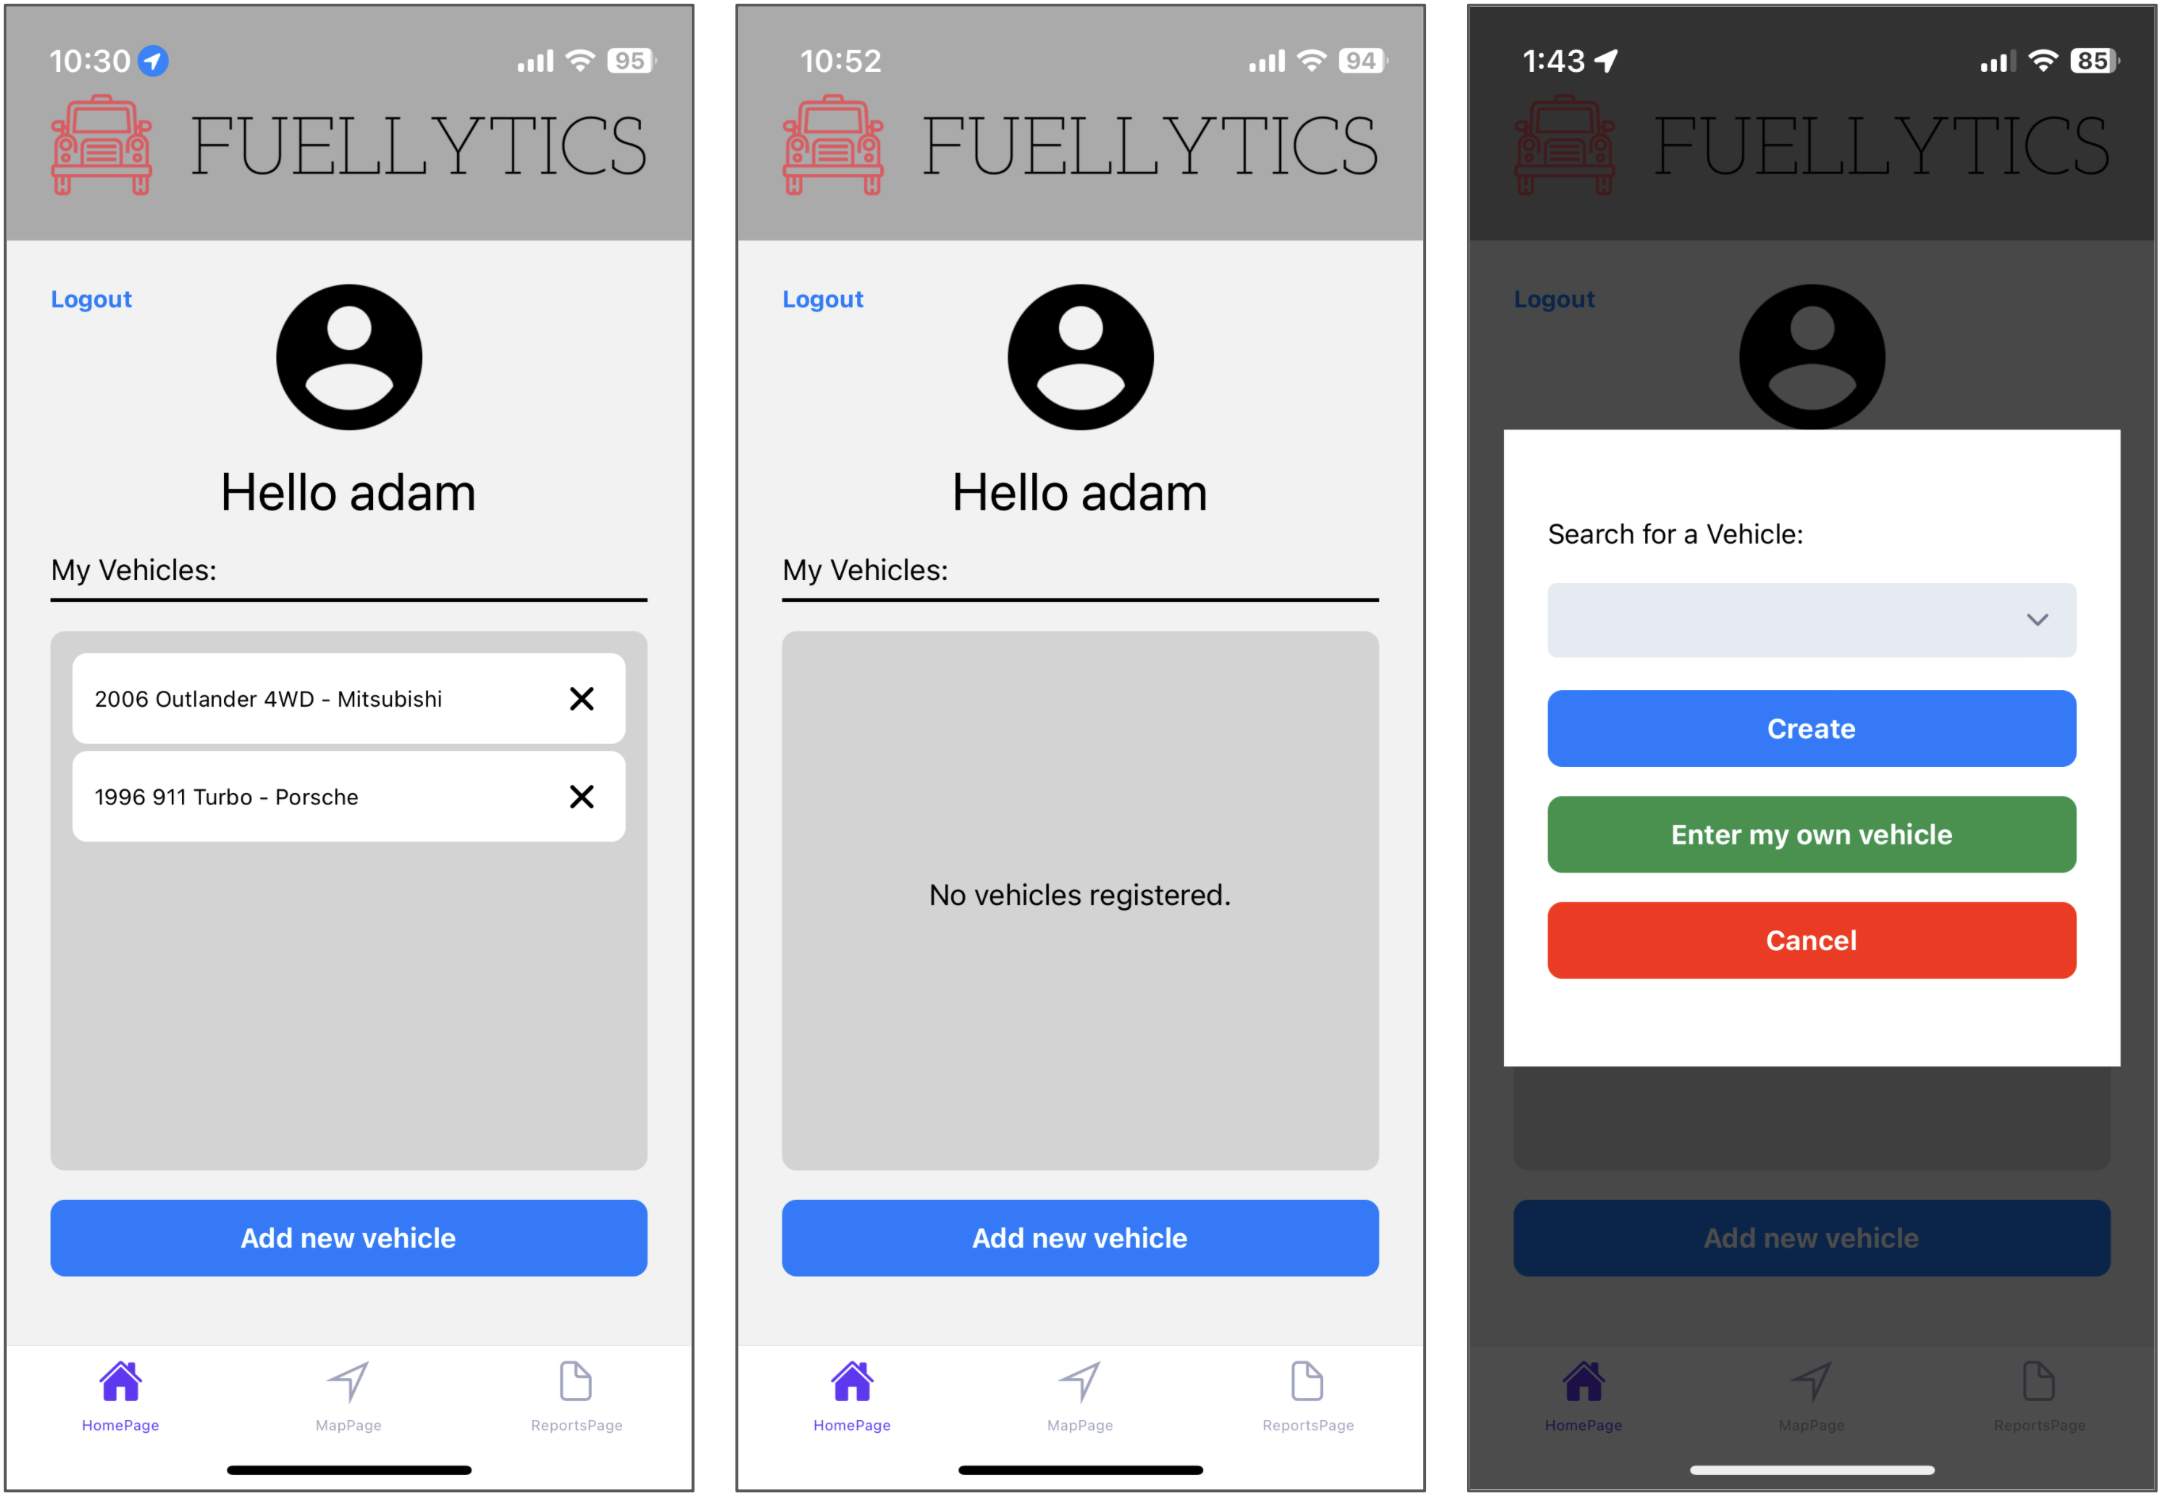
\includegraphics[width=16.5cm]{img/homepage.png}}
\caption{\label{fig:reports} REPLACE FIGURE WITH IMAGES OF REPORTS PAGE.}
\end{figure}


\section{Lessons learned}

One of the most challenging technical aspects of this project was the alignment of the smartphone axes with the frame of the vehicle.  This is necessary to be able to extract the speed and acceleration of the vehicle and enable the fuel consumption calculation.  Since the smartphone is not fixed in the vehicle and can rotate arbitrarily at any time, the orientation parameters describing the relative vehicle-smartphone orientation must be constantly updated and corrected.  The simplest method, and our initial approach, is to utilize the device orientation provided by the iOS and Android operating systems, however, this was found to be unstable and inadequate for our application.  After much testing, our finalized method utilizes the Madgwick AHRS algorithm \reflabel{madgwick} to combine accelerometer, gyroscope, and magnetometer information and provide orientation of the smartphone with respect to the local level frame.  This is then combined with the GNSS-provided heading to obtain the desired orientation parameters.  This algorithm is fast enough for real-time use, but some inaccuracies arise from the magnetic interference of the metal and electrical components of the vehicle.  As such, our algorithm heavily relies on GNSS-provided navigation parameters to provide corrections to the INS-provided navigation solution.

\section{Conclusion}
 
\section{References}

\begin{footnotesize}

\refinit{canadaghg} ``Greenhouse Gas Emissions: Canadian Environmental Sustainability Indicators,'' \textit{Environment and Climate Change Canada}, 2022. Available: \url{https://www.canada.ca/en/environment-climate-change/services/environmental-indicators/greenhouse-gas-emissions.html}

\refinit{reactnative} React-Native, \textit{Meta Platforms, Inc.}, \url{https://reactnative.dev}

\refinit{django} Django, \textit{Django Software Foundation}, \url{https://www.djangoproject.com}

\refinit{transport-emissions} ``Transport, Energy and CO2,'' \textit{International Energy Agency}, Paris, France, 2009. Available: \url{https://www.iea.org/reports/transport-energy-and-co2}

\refinit{oil-based-transport} ``Transport,'' \textit{International Energy Agency}, Paris, France, 2022. Available: \url{https://www.iea.org/reports/transport}

\refinit{driving-style} ``Techniques for Drivers to Conserve Fuel,'' \textit{U.S. Department of Energy}, \url{https://afdc.energy.gov/conserve/behavior_techniques.html}

\refinit{fuel-force} FuelForce Fuel Management Systems, \textit{Multiforce Systems}, \url{https://info.gartnerdigitalmarkets.com/multiforce-gdm-lp?channel=capterra}

\refinit{triscan} Triscan Systems, \textit{Triscan Group Limited}, \url{https://www.thetriscangroup.com}

\refinit{fuelly} Fuelly, \textit{Fuelly, LLC}, \url{https://www.fuelly.com}

\refinit{fuelline} C. Olafson, E. Johston, B. Masciotra, and Y. Mo. \textit{FuelLine}, \url{https://fuel-line.fly.dev/}

\refinit{myearth} ``MyEarth - Track carbon savings,'' \textit{University of Wisconsin}, \url{https://play.google.com/store/apps/details?id=com.ionicframework.myearthapp496614&hl=en_CA&gl=US}

\refinit{capture} ``Carbon Footprint \& CO2 Tracker,'' \textit{The Capture Club}, \url{https://play.google.com/store/apps/dev?id=7417037584465272817&hl=en_CA&gl=US}

\refinit{main-paper}  Q. Zhao, Q. Chen, and L. Wang. ``Real-Time Prediction of Fuel Consumption Based on Digital Map API,'' \textit{Applied Sciences}, vol. 9, no. 7, p. 1396, 2019. \url{https://doi.org/10.3390/app9071369}

\refinit{tank2wheel} C. M. Silva, G. A. Goncalves, T. L. Farias, and J. M. C. Mendes-Lopes. ``A tank-to-wheel analysis tool for energy and emissions studies in road vehicles,'' \textit{Science of The Total Environment}, vol. 367, no. 1, pp. 441-447, 2006. \url{https://doi.org/10.1016/j.scitotenv.2006.02.020}

\refinit{analytic-fc} M. Ben-Chaim, E. Shmerling, and A. Kuperman. ``Analytic Modeling of Vehicle Fuel Consumption,'' \textit{Energies}, vol. 6, no. 1, pp. 117-127, 2013. \url{https://doi.org/10.3390/en6010117}

\refinit{wvu-ai} S. Katreddi and A. Thiruvengadam. ``Trip Based Modeling of Fuel Consumption in Modern Heavy-Duty Vehicles Using Artificial Intelligence,'' \textit{Energies}, vol. 14, no. 24, p. 8592, 2021. \url{https://doi.org/10.3390/en14248592}

\refinit{fc-phone} Y. Yao, X. Zhao, C. Liu, J. Rong, Y. Zhang, Z. Dong, and Y. Su. ``Vehicle Fuel Consumption Prediction Method Based on Driving Behavior Data Collected from Smartphones,'' \textit{Journal of Advanced Transportation}, vol. 2020, 2020. \url{https://doi.org/10.1155/2020/9263605}

\refinit{madgwick} S. O. H. Madgwick. ``AHRS algorithms and calibration solutions to facilitate new applications using low-cost MEMS,'' Ph. D. dissertation, University of Bristol, England, 2014. Available: \url{https://ethos.bl.uk/OrderDetails.do?uin=uk.bl.ethos.681552}

\end{footnotesize}


\end{document}